\documentclass[/Users/ikedahajime/GitHub/reserch/master_report/thesis]{subfiles}
% このファイル内だけのコマンド
\begin{document}
% \chapter{結果}
\section{CABPの結果}\label{sec:result_cabp}
\secref{sec:result_abp}では、 iABP を閉じ込めた時に発生する流れについて述べた。
その結果、系を高密度にした時系全体の運動方向が揃う状態を見ることができた。しかし、その結果についてはノイズが大きく、
角度方向の安定した流れを見ることができなかった。

本節では、ノイズのないモデルとして高密度のCABPを用い、円形領域に閉じ込めた時の結果を示す。%小説での結果のreview
\subsection{系全体のダイナミクス}\label{subsec:CABPdinamicse}
まず、系全体の流れについて議論する。はじめに、規格化された角運動量の時間変化を見る。
\figref{fig:CABP_V_timedep}はパラメータを変化させた時の規格化された角運動量$V$の時間依存性を表すグラフである。
この図におけるパラメータは密度$\varphi=1.209$、$R=10$である。
代表的なパラメータとして(a)は$R_{\Omega}=0.1$、(b)は$R_{\Omega}=10$、(c)は$R_{\Omega}=1000$
を選んだ。3つの図を比較すると、まず$R_{\Omega}$が小さい(a)では$V$の
絶対値が小さく、各粒子がそれぞれ異なる方向へ運動しており、系全体での渦が生じていないことが分かる。
次に$R_{\Omega}$を大きくした(b)では$V$の絶対値は1に近づいており、またその符号は規則正しく正負に振動している。%???
これは粒子全体が一方向に回転していることを示しており、系全体が渦をなして回転し、その方向は周期的に反転する
ことがわかる。
最後により$R_{\Omega}$を大きくした(c)を見ると、$V$は時間によらず1で一定であり、この領域では粒子全体が1つの渦となって、
定常的な流れをなしていることがわかる。ここでは、(a)のように$V$の絶対値が小さく粒子が一方向に進まない領域を乱雑相、(b)のように$V$の絶対値が
1に近く、その符号が正負に振動している領域を振動相、(c)のように$V$の値が時間によらず1で一定の領域を定流相と呼ぶことにする。



\begin{figure}
    \centering
    \begin{tabular}{c}
    % ----- image 1 =====
        \begin{minipage}{0.3\hsize}
            \text{(a)}
            % \centering
            \includegraphics[width=\textwidth]{img/hloabp/figscompANIME/onesR9.963lo1.209Ms0.0ta0Rc0.1Rbit0.0v021.pdf}
        \end{minipage}
    % ----- image 2 =====
        \begin{minipage}{0.3\hsize}
            \text{(b)}
            % \centering
            \includegraphics[width=\textwidth]{img/hloabp/figscompANIME/onesR9.963lo1.209Ms0.0ta0Rc10Rbit0.0v021.pdf}
        \end{minipage}
    % ----- image 3 =====
        \begin{minipage}{0.3\hsize}
            \text{(c)}
            % \centering
            \includegraphics[width=\textwidth]{img/hloabp/figscompANIME/onesR9.963lo1.209Ms0.0ta0Rc1000Rbit0.0v021.pdf}
        \end{minipage}
    \end{tabular}
    \caption[Four sample images]
    {
        円の中に拘束された高密度CABPにおける$V(t)$の時間依存性。(a) $R_{\Omega}=0.1$ (b) $R_{\Omega}=10$ (c) $R_{\Omega}=1000$ で、
        $R=10、\varphi=1.209$。
        $R_{\Omega}$を大きくするにつれて、振幅が大きくなり、また定常的な流れへと遷移していることがわかる。
    }
    \label{fig:CABP_V_timedep}
\end{figure}

これらの相を定量的に評価するため、$V(t)$の時間平均を考える。\figref{fig:vabs_vave_state}(a)、(c)は$V$の絶対値の平均値、
(b)、(d)は$V$の平均値と$R_\Omega$のグラフである。横軸は$R_{\Omega}$で、横軸のみ対数軸になっている。
各図における異なるグラフは異なる系の半径$R$を表す。
図から、いずれも$R_\Omega$を大きくするにつれて大きくなることがわかる。
この量を元にして書いた相図が\figref{fig:vabs_vave_state}(e)である。
縦軸は$R$、横軸は$R_\Omega$で、
両方の軸は対数である。$\langle |\bar{V}| \rangle<0.8$かつ$\langle \bar{V} \rangle<0.8$の点を青色、
$\langle |\bar{V}| \rangle>0.8$かつ$\langle \bar{V} \rangle<0.8$の点を緑色、
$\langle |\bar{V}| \rangle>0.8$かつ$\langle \bar{V} \rangle>0.8$の点を赤色にしてプロットした。
この相図を見ると、系の半径$R$の値に関わらず$R_\Omega$が大きくなると、系は乱雑相、振動相、定流相の順に遷移していくことが分かる。

この遷移のメカニズムについて明らかにするため、\figref{fig:vabs_vave_state}(a)、(b) をスケールする。グラフをスケールすることで、
それらが重なった場合にその遷移を引き起こす仕組みについて考えることができる。
これらの結果をスケールした結果が\figref{fig:vabs_vave_state}(c)、(d)である。
(c)は横軸を$\xi_\bot/R \propto R_\Omega^{1/2}/R$\cite{kurodaLongrangeTranslationalOrder2024}で、
(d)は横軸を$R_\Omega/R$でそれぞれスケールした。このようにスケールすると各半径のグラフが重なる。

まず$\bar{|V|}$について注目する。このオーダーパラメータは全粒子の運動方向がどの程度揃っているのかについて判別する量で、系の協同運動に関係する量である。
ここで、相関長と協同運動との関係について考える。ここで、相関長とはバルク系における変異相関関数の相関長のことを指し、
この長さは渦の大きさに関係する量である。この系においては、黒田らによる先行研究において相関長が研究されており\cite{kurodaLongrangeTranslationalOrder2024}、
相関長$\xi_\bot$が$R_\Omega^{1/2}$に比例することが分かっている。
\figref{fig:vabs_vave_state}(c) は横軸をこの相関長$\xi_\bot$と円の半径$R$との比によってスケールしている。
これによって全ての$R$におけるグラフが重なっており、これはこのパラメータが相関長$\xi_\bot$と半径$R$の比によって変化していることが読み取れる。
また、$R\simeq \xi_\bot$に注目すると、この領域で$\bar{|V|}$が大きくなっている。つまり、バルク系における相関長の大きさが拘束している円の半径と同等になったときに
全ての粒子が同じ方向に向かって運動する協同的な運動を示す。
これは実験系や、複雑な相互作用を持つ理論系における結果と同様の結果である。%TODO*cite



\begin{figure}
    \centering
    \begin{tabular}{c}
        \begin{minipage}{0.3\hsize}
            % \centering
            \text{(a)}
            \includegraphics[width=\textwidth]{img/chiral/HAMLOD3_RAT40/abs_vlog_x.pdf}
        \end{minipage}
            \begin{minipage}{0.3\hsize}
                % \centering
                \text{(b)}
                \includegraphics[width=\textwidth]{img/chiral/HAMLOD3_RAT40/sumvlog_x.pdf}
        \end{minipage}\\
        \begin{minipage}{0.3\hsize}
            \text{(c)}
            \includegraphics[width=\textwidth]{img/chiral/HAMLOD3_RAT40/abs_vlog_xdivide_Rx_sqrt_2.pdf}
        \end{minipage}
        \begin{minipage}{0.3\hsize}
            \text{(d)}
            \includegraphics[width=\textwidth]{img/chiral/HAMLOD3_RAT40/sumvlog_xdivide_R.pdf}
        \end{minipage}\\
        \begin{minipage}{0.5\hsize}
            \text{(e)}
            \vfill
            \includegraphics[width=\textwidth]{img/chiral/HAMLOD3_RAT40_diagram.pdf}
        \end{minipage}
    \end{tabular}
    \caption[Four sample images]
    {
        $V$の時間平均の値。(a)、(c)は$V$の絶対値の平均値、(b)、(d)は$V$の平均値のグラフ。
        横軸は$R_{\Omega}$で、横軸のみ対数軸である。
        (c)は横軸を$\xi_\bot/R \propto R_\Omega^{1/2}/R$\cite{kurodaLongrangeTranslationalOrder2024}で、
        (d)は横軸を$R_\Omega/R$でそれぞれスケールしてある。


        (e)は$\langle |\bar{V}| \rangle$と$\langle \bar{V} \rangle$の値を元にした相図。
        横軸は$R_\Omega$、縦軸は$R$であり、両軸は対数軸。
        $\langle |\bar{V}| \rangle<0.8$かつ$\langle \bar{V} \rangle<0.8$の点を青色、
        $\langle |\bar{V}| \rangle>0.8$かつ$\langle \bar{V} \rangle<0.8$の点を緑色、
        $\langle |\bar{V}| \rangle>0.8$かつ$\langle \bar{V} \rangle>0.8$の点を赤色にしてプロットしている。
        図中の点線は$R=\xi_\bot\propto R_\Omega^{1/2}$を、実線は$R\propto R_\Omega$を
        表す。
    }
    \label{fig:vabs_vave_state}
\end{figure}
続いて、振動相と定流相の間の遷移について考える。この遷移は\figref{fig:image_cabp_in_tube}のように、
一つの粒子が幅$1\sigma$の幅を持つ、半径$R$のリングの中に閉じ込められている状態を考えることで理解することができる。

ここで、極座標におけるこのような CABP について考える。この粒子座標のx軸に対する角度を$\theta_r$、
自己駆動力の進行方向とx軸の軸のなす角度を$\theta_a$、これらの角度の差を$\theta_{ra}=\theta_a-\theta_r$と置く。
この粒子が$0<\theta_{ra}<\pi$である時間を$t_{+}$、$\pi < \theta_{ra}<2\pi$である時間を$t_{-}$と置く。
この時、粒子は$t_+$の間反時計回りに、$t_-$の間は時計回りに運動する。
$R_\Omega$を変化させた時のこの粒子の動きについて考える。
まず、$R_\Omega$が十分小さい時(\figref{fig:image_cabp_in_tube}(a))、自己駆動力がその角度を$\pi$だけ変えるためにかかる時間は十分早く、
その時間における粒子の変位$\delta \theta_r$は十分小さい。この時、$\delta \theta_{ra}\simeq\delta \theta_a$であるため、
$t_+\simeq t_-$となる。よって、このような領域では粒子は規則正しく振動する。

$R_\Omega$を大きくすると(\figref{fig:image_cabp_in_tube}(b))、自己駆動力がその角度を$\pi$だけ変えるためにかかる時間が長くなる。
その間自己駆動力による速度は変わらないため、粒子の変位$\delta \theta_r$は有限の値を持つ。
そのため、$t_+$である条件は、$\theta_{ra}=0$である時刻を$t_0$として、$\theta_{ra}(t_0)=0<\theta_{ra}(t)<\theta_{ra}(t_0+t_+)=\pi$
、つまり$\theta_{r}(t_0)<\theta_a(t)<\pi+\delta\theta_r(t_+)+\theta_r(t_0)$となる。
これによって$t_+$である時間は$R_\Omega$が大きくなるにつれて$\delta \theta_r$だけ長くなり、
反時計回りの回転が増えていく。





\begin{figure}
    \centering
    \begin{tabular}{c}
        \begin{minipage}{0.4\hsize}
            \text{(a)}
            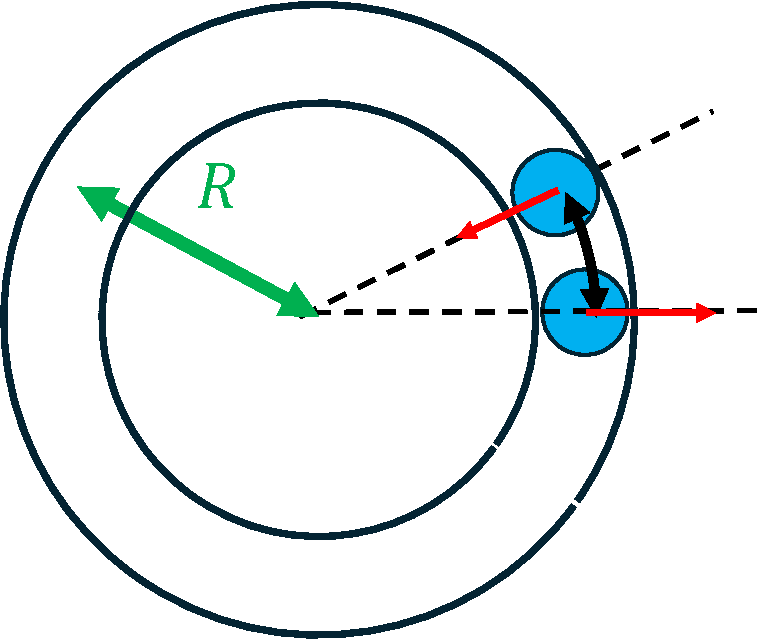
\includegraphics[width=\textwidth]{img/chiral/fig_state/cabp_idou_small_4.pdf}
        \end{minipage}
        \begin{minipage}{0.4\hsize}
            \text{(b)}
            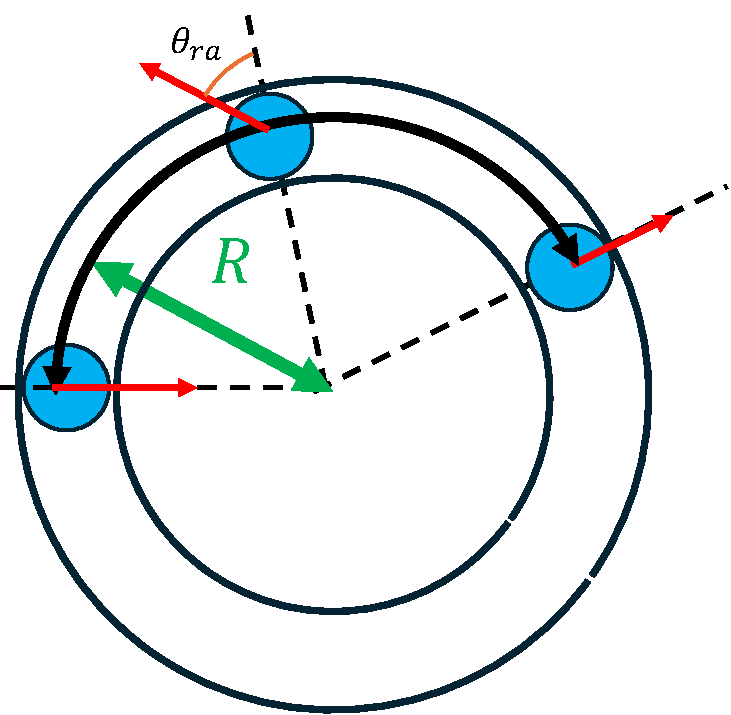
\includegraphics[width=\textwidth]{img/chiral/fig_state/cabp_idou_large_5.pdf}
        \end{minipage}
    \end{tabular}
    \caption[Four sample images]
    {
        狭いチューブの中に入った入った一粒子 CABP の模式図。(a) $R_{\Omega}$が小さくその場で振動する場合
        (b) $R_\Omega$が大きくなり、一周する直前の状態。粒子から出ている矢印はそれぞれの粒子が持つ自己推進の方向を表す。
        これらの図では各粒子がチューブの中で振動する様子を表している。
        }
        \label{fig:image_cabp_in_tube}
    \end{figure}

これは実際に一粒子状態について解析計算をすると分かる。
% 1粒子CABPは、\equref{eq:eom_CABP_1}、\equref{eq:eom_CABP_2}から以下のように表される。
% \begin{eqnarray}\label{eq:eom_CABP_1}
%     \dot{\bm{r}_i}(t) &=& \frac{1}{\zeta} \bm{F}_{wall}(t)+v_0 \bm{e}(\theta_a (t))
% \end{eqnarray}
% \begin{eqnarray}\label{eq:eom_CABP_2}
%     \dot{\theta_i }(t) &=& \Omega
% \end{eqnarray}
リング状の壁に閉じ込められた1粒子CABPは、動径方向の速度が0になる。
そのため、この方程式は\equref{eq:eom_CABP_1}、\equref{eq:eom_CABP_2}から極座標を用いて以下のように表される。
\begin{align}
    v_r&=0\\
    v_t&=v_0 \sin(\theta_a-\theta_r)\\
    \dot{\theta_a}&=\Omega
\end{align}
ここで、$v_r$は方線方向、$v_t$は角度方向の粒子速度である。$\theta_r$は粒子ベクトル$\bm{r}$とx軸正の向きとのなす角であり、
$v_t=R\dot{\theta_r}$。
放線方向の軸と自己駆動の方向がなす角$\theta_{ra}$は、
\begin{align}
    \dot{\theta_{ra}}&=\dot{\theta_a}-\dot{\theta_r}\\
    &=\Omega-\frac{v_0}{R}\sin \theta_{ra}
\end{align}
となる。
% TODO:ratrをいい変数にする
これは1階微分方程式なので解析的に解けて、粒子の回転半径$R_\Omega$と円の半径$R$の比を$r_{R_\Omega R}$とおくと以下のようになる。
\begin{equation}
    \theta_{ra}=
    \begin{cases}
        2 \arctan(-r_{R_\Omega R}+\sqrt{1-r_{R_\Omega R}}\tan (\frac{\sqrt{1-r_{R_\Omega R}^2}}{2}\Omega t))&(r_{R_\Omega R}<1)\\
        2 \arctan(1-\frac{2}{\Omega t}) &(r_{R_\Omega R}=1)\\
        2 \arctan(r_{R_\Omega R}+\sqrt{r_{R_\Omega R}^2-1}\tanh(-\sqrt{r_{R_\Omega R}^2-1}\Omega t))& (r_{R_\Omega R}>1)
    \end{cases}
\end{equation}
平衡化すると、
\begin{equation}\label{eq:cabp_single_ring}
    \theta_{ra}=
    \begin{cases}
        2 \arctan(-r_{R_\Omega R}+\sqrt{1-r_{R_\Omega R}}\tan (\frac{\sqrt{1-r_{R_\Omega R}^2}}{2}\Omega t))&(r_{R_\Omega R}<1)\\
        \frac{\pi}{2} &(r_{R_\Omega R}=1)\\
        2 \arctan(r_{R_\Omega R}+\sqrt{r_{R_\Omega R}^2-1})& (r_{R_\Omega R}>1)
    \end{cases}
\end{equation}

この式から、一粒子における$V$の時間平均$\bar{V}$について求める。
$V$の値は、$0<\theta_{ra}<\pi$の時 1 、$\pi<\theta_{ra}<2\pi$の時 -1 になる。
\equref{eq:cabp_single_ring}から、この値は周期性を持つので、時間平均を求めるためには一周期分について時間平均すれば良い。
したがって、
\begin{align}
    \bar{V}&=
\end{align}


この式からも分かるように、$R_\Omega<R$の領域については粒子は振動運動を示し、
$R_\Omega>R$においては一定の速度で回り続ける。

これを元に\figref{fig:vabs_vave_state}(d) について考える。
図においては横軸を$R_\Omega^1$と$R$の比でスケールしている。
このことから、振動相と定流相の間の遷移は$R_\Omega^1$と$R$の比によって変化していることが分かる。
これは一粒子状態である\equref{eq:cabp_single_ring}における変化と定性的に等価であるが、その遷移する点は
$R\simeq R_\Omega$から離れている。これは粒子間の相互作用によって粒子の速度が遅くなり、実行的な
自走速度が小さくなったためであると考えられる。
また、この結果は Caprini らによる研究\cite{capriniSelfrevertingVorticesChiral2024}と同様の原理に基づいて
遷移していると考えられる。

これらの考察を元にして相図\figref{fig:vabs_vave_state}(e)にそれぞれの層を分ける線を引いた。
図中の点線は$R=\xi_\bot\propto R_\Omega^{1/2}$を、実線は$R= R_\Omega/15$を表す。
この図からも分かるように、$R=\xi_\bot\propto R_\Omega^{1/2}$の線で乱雑相と振動相が、
$R\propto R_\Omega$の線で振動相と定流相が分けられることがわかる。
%周期(時間依存性)
%全体うず(相図)
%ふくうず
\subsection{内部に発生する渦}
\subsecref{subsec:CABPdinamicse}では系全体の流れについて調べた。
続いて、円の中に発生する渦について調べる。\figref{fig:CABP_coor}は$R=20、\varphi=1.209$における渦度場と$\phi_6$の
スナップショットである。これらの図を見ると、を見ると、乱雑相において、円の中で複数の渦が生まれているように
見える。実際に渦度を見ると、複数の、粒径よりも大きな渦が発生していることがわかる。
\begin{figure}
    \centering
    \begin{tabular}{c}
        \begin{minipage}{0.45\hsize}
            \text{(a)}
            \includegraphics[width=\textwidth]{img/chiral/HAMLOD3_RAT40/volR20_Rc0.1.pdf}
        \end{minipage}
        \begin{minipage}{0.45\hsize}
            \text{(b)}
            \includegraphics[width=\textwidth]{img/chiral/HAMLOD3_RAT40/fai6R20_Rc0.1.pdf}
        \end{minipage}\\
        \begin{minipage}{0.45\hsize}
            \text{(c)}
            \includegraphics[width=\textwidth]{img/chiral/HAMLOD3_RAT40/volR20_Rc1.0.pdf}
        \end{minipage}
        \begin{minipage}{0.45\hsize}
            \text{(d)}
            \includegraphics[width=\textwidth]{img/chiral/HAMLOD3_RAT40/fai6R20_Rc1.0.pdf}
        \end{minipage}\\
        \begin{minipage}{0.45\hsize}
            \text{(e)}
            \includegraphics[width=\textwidth]{img/chiral/HAMLOD3_RAT40/volR20_Rc100.0.pdf}
        \end{minipage}
        \begin{minipage}{0.45\hsize}
            \text{(f)}
            \includegraphics[width=\textwidth]{img/chiral/HAMLOD3_RAT40/fai6R20_Rc100.0.pdf}
        \end{minipage}
    \end{tabular}
    \caption[CABP_coor]
    {
        高密度CABPのスナップショット。(a)、(c)、(d) は渦度場のスナップショットであり、矢印は各粒子の速度ベクトルを表す。
        (b)、(d)、(f) は粒子の$\phi_6$である。各図において、パラメータは$R=20、\varphi=1.209$とし、
        (a)、(b) では$R_\Omega=0.1$、(c)、(d) では、$R_\Omega=1$、
        (e)、(f) では$R_\Omega=100$を用いた。その他のパラメータにおけるスナップショットは付録\ref{chap:cabp_snapshot}にまとめた。
    }
    \label{fig:CABP_coor}
\end{figure}
この小さな渦を定量的に評価するため、方位角成分の運動量運動量を見る。\figref{fig:chiral_vel_modes}は方位角成分の運動量
を$R_\Omega$の関数としてプロットしたものである。横軸は\figref{fig:vabs_vave_state}(c)と同様に相関長を半径で割った量
$\xi_\bot/R$でそれぞれスケールしており、対数軸にとっている。

この系では$R_\Omega$が大きくなるに従って粒子の速度は遅くなる。
方位角成分の運動量は速度の2乗に比例するため、生のデータを見ると粒子速度の効果によって渦の生成による効果が隠される。
この影響を避けるため、ここでは30次の運動量まで計算して、0次から30次までの総和で割った量をプロットした。
\figref{fig:chiral_vel_modes}(a)は0次、(b)は1次、(c)は2次、(d)は3次の方位角成分の運動量を表す。

\begin{figure}
    \centering
    \begin{tabular}{c}
        \begin{minipage}{0.4\hsize}
            \text{(a)}
            \includegraphics[width=\textwidth]{img/chiral/HAMLOD3MORE_RAT40/vel_modes_0log_xdivide_Rx_sqrt_2.pdf}
        \end{minipage}
        \begin{minipage}{0.4\hsize}
            \text{(b)}
            \includegraphics[width=\textwidth]{img/chiral/HAMLOD3MORE_RAT40/vel_modes_1log_xdivide_Rx_sqrt_2.pdf}
        \end{minipage}\\
        \begin{minipage}{0.4\hsize}
            \text{(c)}
            \includegraphics[width=\textwidth]{img/chiral/HAMLOD3MORE_RAT40/vel_modes_2log_xdivide_Rx_sqrt_2.pdf}
        \end{minipage}
        \begin{minipage}{0.4\hsize}
            \text{(d)}
            \includegraphics[width=\textwidth]{img/chiral/HAMLOD3MORE_RAT40/vel_modes_3log_xdivide_Rx_sqrt_2.pdf}
        \end{minipage}
    \end{tabular}
    \caption[Vel_modes]
    {
        角運動量成分の運動量。(a) $\langle m_0 \rangle$ (b) $\langle m_1 \rangle$ (c) $\langle m_2 \rangle$ (d) $\langle m_3 \rangle$。
        ただし、各パラメータにおける粒子速度の違いによる影響を避けるため、$n=0$から$n=30$までのモードの和で割ることで規格化している。
        横軸は相関長$\xi_\bot/R$\cite{kurodaLongrangeTranslationalOrder2024}でスケールしており、対数軸を使っている。
    }
    \label{fig:chiral_vel_modes}
\end{figure}

まず\figref{fig:chiral_vel_modes}(a)は0次の方位角成分の運動量であり、この量は系全体の渦について表すモードであるため、
\figref{fig:vabs_vave_state}(c)と同様の性質を持つ量について表しており、それと同様に$R\simeq\xi_\bot$付近でパラメータの値が大きくなっている。
\figref{fig:chiral_vel_modes}(b)(c)(d)はそれぞれ1次、2次、3次の方位角成分の運動量で、これらは渦が2個、4個、8個あることを示す。
それぞれのグラフを見ると、いずれも$\xi_\bot/R$でそれぞれスケールした時にそれぞれのグラフが重なっている。
\subsecref{subsec:CABPdinamicse}と同様の議論を元にすると、
これらの量が相関長と円の半径の比によって変化していることがわかる。
また、これらの量はいずれも1つのピークを持っている。このピークはそれぞれのパラメータに対応する数の渦が多く現れる場所を示す。
そのピークの位置は次数が大きくなるにつれて$R_\Omega$が小さく
なる方向へと動いていることがわかる。
これは小さな渦の発生が、系全体の渦の場合と同様に相関長と円の半径の比によって支配されていることを示す。



ここで、\figref{fig:CABP_coor}に再度注目する。$\phi_6$に注目すると、円の中心付近ではその絶対値が1に近く、
ほとんどの粒子が結晶構造をなしているものの、一部に血管があることが分かる。これは$R_{\Omega}=100$の渦が1つの状態だけでなく、
$R_{\Omega}=0.1、1$の渦が複数存在する状態においても結晶構造をなしている。つまり、これらの系では
粒子配置を壊すことなく速度が渦をなしていると言える。
これは興味深い事実であるが、この事実に対する定量的な解析を行うことはできなかった。
\end{document}
